
\section{Realisierung ( \textasciitilde{} 20- 30 Seiten )}
\label{sec:orgheadline54}
In diesem Kapitel soll vorgestellt werden, was in dem Zeitraum dieser
Bachelorarbeit erreicht wurde. Es soll die Funktionalität des Editors
anhand von Screenshots vorgestellt werden und die Architekur der Anwendung, die selbst nach
Flow Design umgesetzt wurde. 

Als Arbeitstitel für die Anwendung wurde der Name Dexel gewählt.

\subsection{Übersicht über die unterschiedlichen Projekte}
\label{sec:orgheadline5}

Die Anwendung besteht aus einer Solution, die aus folgenden Projekten:
(Fußnote: Bei komplexen Funktionalitäten wurde nach TDD (Test Driven Development)
programmiert, bei dem zuerst der Test geschrieben wird, der das zu erwartende
Ergebnis definiert, und anschließend wurd die Methode erst implementiert, diese
Tests werden in einem extra Test-Projekt für jedes Projekt zusammengefasst)

\subsubsection{Dexel.Model / Dexel.Model.Tests}
\label{sec:orgheadline1}
Dieses Projekt beinhaltet alle Datentypen die zur internen Repräsentation
eines Flow Design Diagrammes nötig sind. Außerdem beinhaltet dieses Projekt
statische Manager-Klassen, die das Arbeiten mit den Datentypen vereinfachen.

\subsubsection{Dexel.Editor / Dexel.Editor.Tests}
\label{sec:orgheadline2}
Das Hauptprojekt, das alle anderen Projekte integriert. Hier wurde das IOSP
Prinzip nicht eingehalten. Dieses Projekt hat nicht nur die Aufgabe die
anderen Projekte zu integrieren, sondern beinhaltet selbst den
UI-Sourcecode. Diese Entscheidung wurde gefällt, da ein Extrahieren der UI
in ein anderes Projekt sich als zu schwierig erwies. Eine Lösung dafür zu
finden, wie ein Event aus dem UI mit einer Funktionalität verbunden werden
könnte, aus einem Projekt, welches es selbst nicht, war zeitlich zu
aufwendig. Aus diesem Grund wurde entschieden auf die zusätzliche
Komplexität einer Entkoppelung zu verzichten und der Einfachheit halber
dieses Projekt als UI und integrierendes Projekt zu nutzen.

\subsubsection{Roslyn / Rosyln.Tests}
\label{sec:orgheadline3}
Diese Projekt beinhaltet die Logik zur Erstellung von C\#-Code aus einem Flow
Design. Mircosoft Rosyln ist die Technik, die hier zum Erstellen von Code zum
Einsatz kommt.
Das Flow Design Diagramm muss in Form eines Mainmodels aus dem
Dexel.Model Projekt vorliegen. Aus diesem Grund gibt es eine Abhängigkeit
zwischen diesem Projekt und dem Dexel.Model Projekt. 

Eine Trennung dieser Abhängigkeit wurde versucht umzusetzen indem gegen ein Interface
programmiert wurde, anstatt gegen die konkrete Implementation in
Dexel.Model. Diese Interfaces der Datentypen und Manager-Klassen wurde dann
in ein Contracts-Projekt ausgelagert, von dem alle anderen Projekte abhängig
sein durften. Die zusätzliche Komplexität, Mehraufwand und ein Problem bei
der Serialisierung von Datentypen, bestehend aus weiteren Interfaces als
Properties, machte die Entkoppelung nicht wert und der Beschluss auf die
Interfaces zu verzichten wurde gefällt.

\subsubsection{Dexel.Library}
\label{sec:orgheadline4}
Beinhaltet einige Methoden ( meist Extension-Methoden), die ein Arbeiten
nach Flow Design erleichter. Diese wurden in ein separates Projekt
ausgelagert, damit alle anderen Projekte darauf zugreifen können.

\subsection{Das Model}
\label{sec:orgheadline14}
Um nachfolgende Kapitel der Realisierung und die darin enthaltenden
Codeauschnitte verstehen zu können, braucht es ein Verständnis darüber, wie die
grundlegenden Datentypen des Models aufgebaut sind. Um die Funktionalität der
jeweiligen Datentypten besser zu veranschaulichen, werden in diesem Kapitel
Bilder verwendet, welche die spätere Darstellung des Datentypen in der UI zeigen.

\subsubsection{{\bfseries\sffamily MISSING IMAGES} MainModel}
\label{sec:orgheadline6}
Das MainModel ist, wie der Name schon sagt, das Haupt-Modell, das alle
anderen Modelle per Komposition beinhaltet. Somit kann man eine Objektinstanz
eines MainModels an eine Methode übergeben und diese Instanz beinhaltet alle
Informationen über das aktuelle Flow Design Diagramm. 
Das MainModel beinhaltet alle Funktonseinheiten (\texttt{SoftwareCells}), alle verbindende
Datenströme (\texttt{Connections}) und alle benutzerdefinierten Datentypen (\texttt{DataTypes}).

\begin{verbatim}
[ImplementPropertyChanged]
public class MainModel
{
public List<SoftwareCell> SoftwareCells { get; set; }
public List<DataStream> Connections { get;  set; }
public List<DataType> DataTypes { get; set; } 
}
\end{verbatim}

\subsubsection{{\bfseries\sffamily MISSING IMAGES} SoftwareCell}
\label{sec:orgheadline8}
In Anlehnung an den Gedanken der Softwarezellen-Architekur und den Schluss
daraus, dass auf unterster Ebene eine Funktionseinheit auch als
Softwarezellen gedacht werden kann, wurden Funktionseinheiten als
Softwarezellen bezeichnet.

\begin{verbatim}
[ImplementPropertyChanged]
public class SoftwareCell
{
public Guid ID { get; set; }
public string Name { get; set; }
public Point Position { get; set; }
public List<SoftwareCell> Integration { get; set; }
public List<DataStreamDefinition> InputStreams { get; set; }
public List<DataStreamDefinition> OutputStreams { get; set; }
}
\end{verbatim}

Der Name ist der Name der Funktionseinheit ( der Text, der bei der
Darstellung später innhalb des Kreises erscheint). Dieser wird später per Binding
direkt an die UI gebunden. Aus diesem Grund implementiert dieses Klasse,
genau wie alle anderen des Models, die ImplementPropertyChanged
Funktionalität. Diese bewirkt, dass bei einer Änderung im UI automatisch das
entsprechende Property im Model aktualisiert wird und umgekehrt.

Die Position beschreibt die Position der Softwarezelle innherhalb des
Diagrammes.  

Das Integration Property gibt an, ob diese Softwarezelle eine Integration
ist und welche andere Instanzen von Softwarezellen sie integriert.
Eine leere Liste besagt, dass die Softwarezelle keine Integration ist.

Die Input- und OutputStreams definieren die möglichen ein- und ausgehenden
Datenströme der Softwarezelle. An diese DataStreamDefinitionen können sich DataStreams
verbinden. Dadurch lassen sie die Datenflüsse modelieren.

\begin{enumerate}
	\item {\bfseries\sffamily MISSING IMAGES} DataStreamDefinition
	\label{sec:orgheadline7}
	
	\begin{verbatim}
	[ImplementPropertyChanged]
	public class DataStreamDefinition
	{
	public Guid ID { get;  set; }
	public string DataNames { get;  set; }
	public string ActionName { get;  set; }
	public SoftwareCell Parent { get;  set; }
	public bool Connected { get;  set; }
	}
	\end{verbatim}
	
	Eine Funktionseinheit verfügt über ein oder mehrere ein- und ausgehende
	DataStreamDefinitionen. Diese können verbunden sein oder nicht. Wenn eine
	Verbindung erstellt und gelöscht wird, muss deshalb auch das Connected
	Property immer gesetzt werden, damit das Model valide bleibt.
	Ob eine DataStreamDefinition verbunden ist, oder nicht, ist vorallem später
	für die Darstellung relevant.
	Eine DataStreamDefinition kennt auch die Funktionseinheit, von der sie ein
	Ein- oder Ausgang ist.
	
	Eine weitere grundlegende Eigenschaft ist die Benennung der Daten, die in/aus
	dem Ein-/ Ausgang fließen. Für Ausgänge ist auch die Angabe eines
	Actionnames manchmal nötig. Dieser soll später unterhalb des Pfeiles
	dargstellt werden.
\end{enumerate}

\subsubsection{{\bfseries\sffamily MISSING IMAGES} DataStream (Connections)}
\label{sec:orgheadline9}
Um Datenflüsse zwischen Funktionseinheitn zu beschreiben, bedarf es einer
Verbindungsklasse. Die DataStream-Klasse stellt diese Verbindungsklasse dar.


\begin{verbatim}
[ImplementPropertyChanged]
public class DataStream
{
public Guid ID { get; set; }
public string DataNames { get;  set; }
public List<DataStreamDefinition> Sources { get;  set; }
public List<DataStreamDefinition> Destinations { get;  set; }

}
\end{verbatim}

Ein DataStream hat ein oder mehrere Referenzen an DataStreamDefinition als
Quellen und ein oder mehrere Referenzen an DataStreamDefinition als Ziele.
Um ein Datenstrom zu beschreiben, der aus mehren Quellen Daten bezieht und
an einer Stelle zusammenläuft, benötigt man ein DataStream, der mehrer
Einträge in der Source-Liste besitzt und ein Eintrag in der
Destination-Liste. Diese Datenstrom wäre dann ein Joint-Input.
Ein Datenstrom mit einer Quelle und mehreren Zielen wäre ein Joint-Output ( TODO:
Referenz auf vorheriges Kapitel)

Das DataNames Property stellt den Text dar, der später in der Mitte des
Pfeiles dargestellt werden soll. Eine Änderung dieser Eigenschaft bedarf
einer Aktualisierung der DataNames aller Sources und Destinations.
Eine Aktualisierung muss die optionalen Pipe-Notation kennen und
entsprechend dieser die Ein und Ausgänge akutalisieren.

Der akutelle Stand der UI kann akutell nur Datenflüsse mit einer Quelle und
einem Ziel darstellen.

\subsubsection{DataType}
\label{sec:orgheadline10}

\begin{verbatim}
[ImplementPropertyChanged]
public class CustomDataType
{
public string Name { get; set; }
public List<SubDataType> SubDataTypes { get; set; }
}

[ImplementPropertyChanged]
public class SubDataType
{
public string Name { get; set; }
public string Type { get; set; }
}
\end{verbatim}

Ein benutzerdefinierter Datentyp besteht aus einem Namen und einer Liste von mehreren
\texttt{SubDataType}-Objekten. 

Ein SubDataType besteht aus einem Namen und den Namen
des Types (zum Beispiel string, int oder auch ein anderen benutzerdefinierten
Datentypen).

\subsubsection{Manager-Klassen}
\label{sec:orgheadline13}
\begin{enumerate}
	\item MainModelManager
	\label{sec:orgheadline11}
	Einer der relevantesten Manager-Klassen ist die MainModelManager-Klasse,
	diese stellt die wichtigsten Funktionalitäten zur Verfügung die mit dem
	Arbeiten des MainModels gebraucht werden. Einige dieser Funktionalitäten
	wären: Verbinden und Trennen von Funktionseinheiten, vorwärts und rückwärts
	Traversieren entlang des Graphen, Hinzufügen und Entfernen einer
	Funktionseinheit von einer Integration, Hinzufügen, Löschen und Duplizieren
	von Funktionseinheiten, oder Teile des Graphen.
	
	\item DataStreamManager
	\label{sec:orgheadline12}
	Diese statische Klasse bietet einige Funktionalitäten, die das Arbeiten mit
	Objekten der DataStream-Klasse vereinfachen soll.
	
	Ein Beispiel hierfür wäre das Ändern des Datanames eines DataStreams. 
	Wie bereits in letzten Abschnitt erwähnt, muss beim Ändern der Daten
	eines Datenflusses auch die Daten seiner Sources und Destinations
	angepasst werden. 
	
	Um dies nochmal zu verdeutlichen, zwei konkrete Beispiele:
	Falls der Datenfluss auf (int)|(string) geändert werden
	soll, muss die Source-DataStreamDefinition auf (int) gesetzt werden und der
	die Destination-DataStreamDefinition auf (string). 
	Falls der Datenfluss auf (double) geändert werden soll, so werden Source
	und Destination Daten auf (double) gesetzt.
	
	Fussnote: Da aktuell nur DataStreams mit einer Source und einer Destination im Editor unterstützt
	werden, wurde akutell auch nur dieses Szenario implementiert. Ändert sich
	diese Einschränkung müsste man sich Gedanken darüber machen, was in diesen
	Fällen zu tun wäre. Ein Option wäre, die Pipe-Notation in diesen Fällen zu
	verbieten. Die UI würde die Daten der DataStreamDefinitionen direkt
	anzeigen und der Benutzer würde diese dann direkt ändern. Der Datenstrom
	selbst würde dann kein eigenes Textfeld besitzen und die Dataname
	Eigenschaft hätte in diesen Fall keine Bedeutung. 
	Vielleicht wäre es dann auch besser im Modell zwei separate Klassen
	anzulegen und die
	einfache DataStream-Klasse hätte anstatt einer Liste von DatastreamDefinitionen nur noch ein einfaches Feld
	für eine Source-DataStreamDefinition und eine Destionation-DataStreamDefinition.
	
	\begin{verbatim}
	public static void ChangeDatanames(DataStream datastream, string newDatanames)
	{
	// update datanames of connection itself
	datastream.DataNames = newDatanames;
	
	// update datanames of DSDs
	TrySolveWithPipeNotation(newDatanames,
	onSuccess: (outputPart, inputPart) =>
	{
	// TODO: doesn't support mutliple sources yet
	datastream.Sources.First().DataNames = outputPart;
	datastream.Destinations.First().DataNames = inputPart;
	},
	onNoSuccess: () =>
	{
	// TODO: doesn't support mutliple destinations yet
	datastream.Sources.First().DataNames = newDatanames.Trim();
	datastream.Destinations.First().DataNames = newDatanames.Trim();
	});
	}
	\end{verbatim}
\end{enumerate}



\subsection{Der Editor}
\label{sec:orgheadline33}
\subsubsection{Vorstellung was erreicht wurde}
\label{sec:orgheadline22}

Die Grundlegenden Basisfunktionen aus Kaptitel 3 wurden größtenteils
implementiert. Hierbei kam WPF als GUI-Framework zum Einsatz.
Im folgendem einige Bilder und Beschreibungen der GUI und Interaktionen.

\begin{enumerate}
	\item {\bfseries\sffamily MISSING IMAGES} Erstellen von Funktionseinheiten, Verschieben, Benennen, Selektieren
	\label{sec:orgheadline15}
	Das Drawing-Board wurde implementiert, auf dem der Benutzer mit einem
	Rechtsklick->Create New Function Unit eine erste Funktionseinheit erzeugen
	kann. Per Drag an Drop kann er diese dann innerhalb des DrawingBoards frei
	verschieben. Mit einer Rect-Selektion ist es mögliche mehrere
	Funktionseinheiten zu Selektieren. Selektierte Funktionseinheiten können
	gemeinsam verschoben, dupliziert und gelöscht werden.
	
	Nach dem Erstellen einer neuen Funktionseinheit, wird diese automatisch
	selektiert und der Tastaturfokus wird in das Textfeld des Kreises gesetzt.
	Durch lässt sich diese Benennen.
	
	Beim Klicken auf den äußeren Teil des Kreises wird die Funktionseinheit
	selektiert. Beim Klicken auf das Textfeld, wechselt der Tastaturfokus auf
	das Textfeld ( ein Mouse-Hover zeigt auch an, über welchen Teil des Kreises
	man sich gerade befindet, auch ein Klicken und Ziehen um sofort ein Teil
	des Textes zu markieren bleibt damit dem Benutzer möglich. Wie er es von
	einem Textfeld gewohnt ist).
	
	
	\item {\bfseries\sffamily MISSING IMAGES} Erstellen/Löschen/Manipulieren von Inputs und Outputs
	\label{sec:orgheadline16}
	Eine Funktionseinheit wird standardmässig mit einem Input und einem Output
	erstellt. Die Daten die aus diesen hinein- oder herausfließen können auf
	dem Textfeld eingetragen werden. Dabei bietet diese Textfeld ein einfaches
	Syntaxhighlighting, dass mit Doppelpunkt getrennte Namen-Type-Paare
	farblich trennt. Auch Symbole wie * | [] () , \ldots{} haben eine eigene Farbe.
	
	Der Action-Name kann unterhalb des Pfeiles eingetragen werden.
	
	Eine Funktionseinheit kann mehr als nur einen Output besitzen.
	Zum Hinfzufügen eines neuen Outputs: Rechtsklick -> Add New Output
	Das Löschen eines Outputs ist durch auch möglich: Rechtsklick auf ein
	Output -> Delete.    
	
	Die Reihenfolge bei mehreren Outputs kann per Drag and Drop verändert werden.
	
	\item {\bfseries\sffamily MISSING IMAGES} Verknüpfen und Trennen von Funktionseinheiten über Drag and Drop
	\label{sec:orgheadline17}
	Wird das Ende eines Pfeiles eines Output auf ein Input Pfeil gedropt, so werden beide
	miteinandern Verbunden. Die Datennamen des Flusses werden bei nicht
	Übereinstimmung der beiden Daten des Input und Outputs mit
	der Pipe-Notation beschrieben. Stimmen beide Überein, kann darauf
	verzichtete werden.
	
	Werden die Daten eines verbundenen Datenflusses geändert, werden die Inputs
	und Outputs mit Berücksichtigung auf die Pipe-Notation angepasst, sodass
	beim Trennen der Beiden Funktionseinheiten, die Änderungen erhalten bleiben.
	
	Ein Drag and Drop eines Outputs direkt auf eine Funktionseinheit: TODO
	
	Durch Drag and Drop eines verbunden Pfeiles auf eine leere Stelle auf dem
	DrawingBoard, kann eine Verbindung getrennt werden. Wird sie auf eine
	anderen Input gedropt, so wird diese als neues Ziel gesetzt und die 
	Verbindung zur vorherigen Funktionseinheit gelöscht. TODO
	
	
	\item {\bfseries\sffamily MISSING IMAGES} Erstellen von Integrationen
	\label{sec:orgheadline18}
	Durch Rechtsklick auf eine Funktionseinheit kann im Kontextmenu der Eintrag
	'Make to Integration of (Pick)' ausgewählt werden. Der Cursor verändert
	sich und wird nun eine andere Funktionseinheit angeklickt, so wird der
	komplette Flow, in der diese Funktionseinheit Teil ist, als zu
	Sub-Flow der Integration genommen.
	
	Das Entfernen eines Flows von einer Integration geschieht indem auf eine
	Funktonseinheit rechtsklickt und dann auf 'Remove from Integration'
	ausgewählt wird. Der komplette zusammenhängede Flow wird dann aus der
	Integration entfernt. 
	
	
	Bei einer Modifikation des Datenflusses innerhalb einer Integration, werden nach
	bestimmten Regeln die nachfolgenden (abgetrennten) Funktionseinheiten
	ebenfalls aus der Integration entfernt. Wird die erste Funktionseinheit
	entfernt, gilt diese Regel nicht.
	
	\item Definieren von Datentypen
	\label{sec:orgheadline19}
	Eigene DatenTypen können auf der rechten Seite des Editors angelegt werden.
	Durch Rechtsklick -> Add New DataType. Außerdem zeigt der obere Button an,
	ob im akutellen Diagramm Datenflüsse mit Daten fließen, die nicht definiert
	sind. ( int, string, double, usw. werden automatisch ignoriert). Ein Klick
	auf diesen erstellt für jeden nicht-definierten Datentyp ein neuen Eintrag.
	Auch Datentypen innerhalb eines eigenen Datentypen werden überprüft, ob sie 
	bekannt sind oder nicht. Bsp. 
	Person 
	name:string
	address:Address  
	
	Der Editor würde überprüfen ob der Address Datentyp definiert wurde oder nicht.
	
	\item {\bfseries\sffamily MISSING IMAGES} Navigation und Shortcuts
	\label{sec:orgheadline20}
	Zur Navigation innerhalb des DrawingBoards wird das Mausrad verwendet.
	Durch Scrollen wird in das DrawingBoard herein und herausgezoomt.
	Durch gedrückthalten des Mausrades (mittlere Maustaste) und Bewegen der
	Maus kann die Ansicht verschoben werden ( das DrawingBoard ist endlos groß)
	
	Ein weiteres Feature besteht darin, dass ab bestimmten Zoom-Stufen die
	Font-Größen der Namen der Funktionseinheiten angepasst werden und die 
	Textfelder der Datenflüsse ausgeblendet werden.
	Außerdem können Textfelder nicht mehr fokusiert werden, was ein einfachers
	Verschieben der Funktionseinheiten ermöglichen soll. Diese Eigenschaft wird
	visuell erkenntlich gemacht, dass die Hintergrundfarbe des Textfeldes bei
	einer selektierten Funktionseinheit nicht mehr dunkel ist.
	Auch der Mousecursor zeigt bei einem Mouse-Over an, dass man nicht mehr in
	das Textfeld klicken kann.
	
	
	\item Weitere Features
	\label{sec:orgheadline21}
	\begin{itemize}
		\item Speichern, Laden, Mergen.
		Speichern und Laden in 3 Dateiformate werden unterstüzt.
		(yaml, json und xml - nach Dateigröße aufsteigend sortiert)
		Auch das Laden eines anderen Flow Design in das akutelle geladene wird 
		mit der Merge-Funktion unterstützt.
	\end{itemize}
	
	
	\begin{itemize}
		\item Unhandled Exception ErrorDialog
		Wird eine Exception geworfen, die nicht behandelt wurde, so wurde eine
		allgemeine Fehlerbehandlung aufgerufen. Das Programm stürzt nicht ab,
		sondern ein Dialog errscheint, mit einem Stacktrace und Informationen
		über die geflogenen Exception. Der Benutzer kann das entscheiden, ob er
		hier das Programm Beenden will, oder weiter den Fehler ignorieren will.
		Der Stacktrace kann gegenenfalls kopiert und an den Entwickler als
		Bugreport zuschicken werden.
	\end{itemize}
	
	
	\begin{itemize}
		\item Help-Window
		Ein kleines einfaches Fenster gibt dem Benutzer einen Überblick über die
		vorhandenen Shortcuts und die Navigation mit der Maus wird erklärt.
	\end{itemize}
\end{enumerate}




\subsubsection{Views / ViewModels}
\label{sec:orgheadline23}
Das Projekt wurde nicht strikt nach MVVM-Regeln (Model-View-ViewModel) 
umgesetzt, jedoch bedient es sich der Idee, das es eine View gibt, die
als Datenkontext ein ViewModel zugewiesen hat. Das zuweisen eines
Datenkontextes erlaubt es Elemente der View an Properties des ViewModels zu
binden. Ein Binding bewirkt, dass sich die UI-Element automatisch updatet,
sobald sich das dazugehörige Property ändert. Eine Änderung einer
Eigenschaft des ViewModels ändert also automatisch die View.

Die GUI besteht aus mehreren Views (xaml-Dateien) und dazugehörigen ViewModels.
Die Aufgabe des ViewModels besteht vorallem darin, ein Model entgegenzunehmen und dieses
darzustellen, bzw. die aktuelle Darstellung zu aktualisieren.

Nach jeder Änderung am Model - zum Beispiel das Hinzufügen einer neuen
Node -  dieses komplet neu zu laden (Löschen und neu Hinzufügen aller
ViewModels, die wiederum ein neu Generieren der UI-Framework-Elemente zur
Folge hatte) erwies sich als nicht sehr performant. 
Ab Diagrammen, mit über 20 Nodes, stieg die Zeit zur Aktualisierung der View
bereits auf mehrere Sekunden an.
Die Lösung bestand darin, nicht einfach stur alles zu Löschen und neu
hinzuzufügen, sondern darin, die Änderungen am Model zu lokalisieren und nur
diese neu zu erstellen, bzw nur die Properties neu zu setzen. Durch
diese Verbesserungen wurde die Performance deutlich gesteigert, sodass
Diagramme mit mehrern hundert Nodes keine spürbaren Perfomanceverluste mit
sich führt. Einzig das Duplizieren von vielen Nodes dauert nach wie vor
mehrere Sekunden. 

\subsubsection{Interaktionen}
\label{sec:orgheadline26}
Wie bereits in Kapitel 2 (Abschnitt Entwurfsmethode) schlägt Flow Design
vor, alle Events als Interaktionen zu bezeichnen und für jedes dieser
Änderungen ein eigenen Flow Design zu erstellen. 
Es bietet sich somit an, alle Interaktionen in einer Klasse zu sammeln.
Diese bietet somit eine Überblick über alle Funktionalitäten der GUI.
Da diese Integrationen sind, sind sie leicht zu verstehen (mit Ausnahmen). Die
Interaktionen rufen Methoden von anderen Klassen auf, die die Operationen am
Mainmodel vereinfachen. Am Ende fast jeder Interaktion wird die \texttt{ViewRedraw}
Methode aufgerufen, die das \texttt{MainViewModel} veranlasst, das Model neu zu
laden und somit die Änderungen der Interaktion in der GUI sichtbar macht.
Deshalb erwies es sich als schlecht, wenn eine Interaktion eine andere
Interaktion aufruft, um ihre Funktionalität umzusetzen. 
Stattdessen war es eine bessere Lösung, den Code der einen Interaktion in
die andere zu Kopieren. Dies wiederspricht zwar dem DRY Prinzip, jedoch eine
Coderedundanz innerhalb von Integrationen stellt sich als nicht sehr schlimm
heraus. Integrationen beinhalten schließlich keine Logik (Fussnote: Beim
Aufruf einer Funktionseinheit, die mehrere Outputs liefert, existiert
eigentlich auch eine Logik in der Integration ( Bsp: IsIntegration: Wenn ja,
dann X wenn nicht, dann Y. Dadurch verlieren Integrationen etwas ihre
Leichtgewichtigkeit und sind nicht mehr ganz so einfach zu verstehen ) und haben eine hohe
Abstraktion.

Beispiel dieser Aussage:
\begin{verbatim}
public static object AppendNewFunctionUnit(FunctionUnit currentFunctionUnit, double offsetX, DataStreamDefinition outputToConnect, MainModel mainModel)
{
var newFunctionUnit = FunctionUnitManager.CreateNew();

newFunctionUnit.Position = currentFunctionUnit.Position;
newFunctionUnit.MoveX(offsetX);

// default IO of new function unit: input of new function unit = output to connect to of current function unit
newFunctionUnit.InputStreams.Add(DataStreamManager.NewDefinition(newFunctionUnit, outputToConnect));
newFunctionUnit.OutputStreams.Add(DataStreamManager.NewDefinition(newFunctionUnit, "()"));
MainModelManager.ConnectTwoDefintions(outputToConnect, newFunctionUnit.InputStreams.First(), mainModel);

mainModel.FunctionUnits.Add(newFunctionUnit);

ViewRedraw();

return newFunctionUnit;
}

public static FunctionUnit CreateNewOrGetFirstIntegrated(FunctionUnit currentFunctionUnit, MainModel mainModel)
{
FunctionUnit @return = null;

currentFunctionUnit.IsIntegration(
isIntegration: () => @return = currentFunctionUnit.IsIntegrating.First(),
isNotIntegration: () =>
{
var newFunctionUnit = FunctionUnitManager.CreateNew();
newFunctionUnit.Position = currentFunctionUnit.Position;
newFunctionUnit.MoveY(100);

newFunctionUnit.InputStreams.Add(DataStreamManager.NewDefinition(newFunctionUnit, currentFunctionUnit.InputStreams.First()));
newFunctionUnit.OutputStreams.Add(DataStreamManager.NewDefinition(newFunctionUnit, "()"));

currentFunctionUnit.IsIntegrating.Add(newFunctionUnit);

mainModel.FunctionUnits.Add(newFunctionUnit);

@return = newFunctionUnit;
ViewRedraw();
});

return @return;
}
\end{verbatim}



\begin{enumerate}
	\item {\bfseries\sffamily MISSING IMAGES} Auswirkungen der beiden Interaktionen (Listing Caption)
	\label{sec:orgheadline24}
	Die \texttt{AppendNewCell} Methode erzeugt eine neue SoftwareCell und und
	verschiebt diese entlang der X Postion.
	Außerdem setzt sie den Input gleich der DataStreamDefinition die
	übergebenen wurde und verbindet diese beiden.
	\texttt{AppendNewCell} wird durch die Tastenkombination Ctrl-Tab ausgelöst, wenn
	sich der Tastaturfokus innerhalb eines Textfeldes einer View einer Softwarecell oder
	DatastreamDefinition befindet. Bei ersterem wird der erste unverbunden Output als der
	DataStreamDefinition genommen, andem die neue SoftwareCell angehängt wird (
	nicht Teil dieser Methode).
	
	Beide Methoden geben eine
	Model-Instanz als \texttt{object} an die GUI zurück. Die GUI-Logik findet dann die
	dazugehörige View und setzt den Focus darauf.
	
	\item Coderedundanzen
	\label{sec:orgheadline25}
	Beide Methoden sind Methoden aus der Interaktions-Klasse, sind werden also
	direkt aus einem Event von der GUI ausgelöst. 
	Beide Methoden haben ähnliche Methodenaufrufe ( Neue Funktionseinheit
	erzeugen, sie auf die gleiche Position zu setzten wie die der übergebenen
	Funktionseinheit, neue Default-Werte für den Output-Stream der neuen
	Funktionseinheit setzen, dem MainModel die neue Funktionseinheit zu geben
	und die Ansicht neu zu zeichnen). Diese könnten in eine neue
	Integration ausgelagert werden, hätte jedoch eine unnötige
	Verschachtelung von Code als Auswirkung. Besser ist es hier die
	Coderedundanz als etwas nicht schlimmes anzusehen und diese zu belassen.
	So ist auf einen Blick ersichtlich, was die Interaktion genau macht, ohne
	im Code herumspringen zu müssen.
\end{enumerate}

\subsubsection{Eigene Tabstop-Logik}
\label{sec:orgheadline31}
Mit Tab und Shift-Tab soll es dem Nutzer möglich sein den Tastaturfokus zu
verändern. Dieses Beispiel zeigt dabei noch einmal, das Coderedundanzen innerhalb
von mehreren Integrationen nichts Schlechtes sein muss.
Außerdem macht es auch deutlich, wie eine etwas komplexerer Integration mit
mehreren verschachteteln Lambda-Ausdrücken in der Praxis aussehen kann.
Auch das Arbeiten mit dem Model und Managerklassen soll
dieses Beispiel dem Leser verdeutlichen.


Der nächsten Tabstop soll nach folgenden Regeln und abhängig vom aktuell
fokusierten Model bestimmt werden:

\begin{enumerate}
	\item {\bfseries\sffamily MISSING IMAGES} FunctionUnit
	\label{sec:orgheadline27}
	Besitzt akutell die View einer FunctionUnit den Tastaturfokus, so soll als
	nächste Stop der erste Datenfluss, der verbunden ist gewählt werden. Ist keiner
	verbunden, wähle als nächsten Tabstop den ersten Output.
	
	\item {\bfseries\sffamily MISSING IMAGES} DataStream
	\label{sec:orgheadline28}
	Der sehr einfache Fall trifft ein, wenn der Fokus aktuell auf einem
	DataStream liegt. Der nächste Stop ist dnn die Ziel-Funktionseinheit des Datenflusses
	
	\item {\bfseries\sffamily MISSING IMAGES} DataStreamDefinition
	\label{sec:orgheadline29}
	Der komplexeste Fall: 
	Zu erst muss überprüft werden, ob es sich um ein Input oder Output
	handelt. Ist es ein Input, so soll als nächster Stop die Funktionseinheit
	selbst zurückgegeben werden, von der die DataStreamDefinition der Input ist. 
	Bei einem Output muss überprüft werden, ob das Ende des Flows erreicht
	wurde, oder nicht. Wird ein verbundener Output entdeckt, wird der
	entsprechende DataStream als nächster Stop zurückgegeben. Ist das Ende
	erreicht, so soll zum Anfang des kompletten Flows gesprungen werden.
	
	\begin{verbatim}
	public static object TabStopGetNext(object focusedModel, MainModel mainModel)
	{
	object @return = null;
	
	focusedModel.TryCast<FunctionUnit>(fu =>
	{
	// prefer connected outputs as next tabstop
	// if no connected take first output defintion if there are any
	fu.OutputStreams.GetFirstConnected(
	foundConnected: connectedDsd => 
	@return = MainModelManager.FindDataStream(connectedDsd, mainModel),
	noConnected: () => 
	@return = fu.OutputStreams.FirstOrDefault());
	});
	
	focusedModel.TryCast<DataStream>(stream =>
	{
	// if focus was inside datastream take its destination function unit as next tabstop
	if (stream.Destinations.Any())
	@return = stream.Destinations.First().Parent;
	});
	
	focusedModel.TryCast<DataStreamDefinition>(dsd =>
	{
	// if focus was inside definition there are two case:
	// is input definition: next tabstop is the function unit of the definition
	// is output definition: in case the end of the flow was reached ( no connected output ) 
	// the next tabstop is the first input definition of the beginning of the whole flow.
	// Is the end not reached go to first connected output datastream
	dsd.CheckIsInputOrOutput( 
	isInput: () => @return = dsd.Parent,
	isOutput: () =>
	{
	dsd.Parent.OutputStreams.GetFirstConnected(
	foundConnected: connectedInput => 
	@return = MainModelManager.FindDataStream(connectedInput, mainModel),
	noConnected: () => // loop tabstop focus when the end is reached
	@return = MainModelManager.GetBeginningOfFlow(dsd.Parent, mainModel)); 
	});
	});
	return @return;
	}
	\end{verbatim}
	
	Analog dazu die Tabstop-Methode in die entgegengesetzte Richtung.
	
	
	\begin{verbatim}
	public static object TabStopGetPrevious(object focusedModel, MainModel mainModel)
	{
	object @return = null;
	
	focusedModel.TryCast<FunctionUnit>(fu => 
	{
	fu.InputStreams.GetFirstConnected(
	foundConnected: connectedDsd => 
	@return = MainModelManager.FindDataStream(connectedDsd, mainModel),
	noConnected: () =>
	@return = fu.InputStreams.FirstOrDefault());
	});
	
	focusedModel.TryCast<DataStream>(stream => 
	{
	if (stream.Sources.Any())
	@return = stream.Sources.First().Parent;
	});
	
	focusedModel.TryCast<DataStreamDefinition>(dsd => 
	{
	dsd.CheckIsInputOrOutput(
	isOutput: () => @return = dsd.Parent,
	isInput: () => 
	{
	dsd.Parent.InputStreams.GetFirstConnected(
	foundConnected: connectedInput =>
	@return = MainModelManager.FindDataStream(connectedInput, mainModel),
	noConnected: () => // loop tabstop focus when the beginning is reached
	@return = MainModelManager.GetEndOfFlow(dsd.Parent, mainModel));
	});
	});
	
	return @return;
	}
	\end{verbatim}
	
	
	\item Erläuterung
	\label{sec:orgheadline30}
	Auf oberster Ebene wird überprüft um welchen Typ von Objekt es sich
	handelt, der aktuell fokusiert ist (Fussnote: Teile davon war Aufgabe der UI und die
	Interaktion bekommt das Model dann als \texttt{object} übergeben. Deshalb bedarf es
	innerhalb der Methode einer Überprüfung des Typen mit TryCast). Nun
	existieren die drei Fälle, abhängig vom übergebenen Typen.
	
	Beachte: Die Sources-Eigenschaft eines DataStream beinhaltet nicht die Funktionseinheit,
	sondern die DataStreamDefinition einer Funktionseinheit. Die eigentliche
	Funktionseinheit enthält die Parent-Eigenschaft der DataStreamDefinition.
	Analog dazu enthält die InputStream- und OutputStream-Eigenschaft der
	FunctionUnit auch nur die DataStreamDefinitionen nicht ein DataStream-Objekt.
	Eine DataStreamDefinition kennt jedoch nicht den Datenfluss, mit dem sie
	verbunden ist. Eine Helfer-Methode der MainModelManager-Klasse stellt
	diese Funktionalität zum Auffinden des DataStream zur Verfügung.
\end{enumerate}

\subsubsection{Was nicht erreicht wurde}
\label{sec:orgheadline32}
Hier einge Auflistung was aus zeitlichen Gründen noch nicht realisiert
wurde, die jedoch für den Einsatz in einem Projekt noch sehr wichtig wären:
\begin{itemize}
	\item Joint-Inputs und Joint Outputs. Dies erfordert Möglicherweise noch einmal
	eine kleine Überarbeitung der Architekur des Models. Auch die Darstellung
	wurde noch nicht realisiert.
	\item Validierung der Synatx - Sowohl eine Validierungslogik als auch eine
	Markierung invalider Synatx innerhalb des Editors wurden nicht realisiert.
	\item Mehr Möglichkeiten die Darstellung übersichtlicher zu gestalten: Auf und
	Zuklappen von Integrationen. Eine 'referenzierte' Kopie einer
	Funktionseinheit zu erstellen, um an anderer Stelle diese weiter zu
	verwenden.
	\item Saubere und eindeutige Darstellung einer Rekursion.
	\item Zuordnen von Funktionseinheiten zu Klassen.
	\item Möglichkeit mehrere Flow Design in einer Art Projekt zu Organisieren.
	Vielleicht auch in Form eines GUI-Skizzen-Editors, indem dann die
	Interaktionen eingetragen werden können.
	\item Autosave und Undo/Redo.
\end{itemize}



\subsection{Roslyn - Generierung von Code aus einem Diagramm}
\label{sec:orgheadline52}

Da eine Flow Design auf unterschiedlichen Weisen im Code umgesetzt werden
kann, mussten hier Entscheidungen getroffen werden, in welchen Fällen
welche Weise gewählt wird. Wird das Projekt weitergeführt, könnte man in
Betracht ziehen, dem Nutzer einige Optionen zur Konfiguration der Generierung
zur Verfügung zu stellen. AKtuell muss er sich jedoch damit abfinden, dass
nur die hier vorgestellte Weise zur Verfügung steht.


\subsubsection{Was erreicht wurde}
\label{sec:orgheadline34}
Die weniger komplexeren Aufgaben wurden vollständig implementiert.
Diese wären: 
\begin{itemize}
	\item Generieung der benutzerdefinierten DatenTypen, und Generierung
	\item der Methodensignaturen anhand einer Funktionseinheit.
\end{itemize}

Die weitaus komplexere Aufgabe: die Generierung der Methoden-Bodys einer Integration wurde nicht
vollständig implementiert.

Um Code zu generieren muss im Editor in der Menuleiste der Eintrag Output
angesteuert werden.
Hier gibt es die Möglichkeit das aktuelle Flow Design in eine Datei zu
generieren, oder aber den Code direkt in das Clipboard zu kopieren( damit man den erzeugten Code bequem an
eine gewünschte Stelle copy-pasten kann).

Außerdem gibt es die Option eine automatische Generierung einzuschalten, die
den Code während der Bearbeitung immer neu generiert und in die Datei
schreibt. So lässt sich das Ergebnis der Generierung während der Bearbeitung
des Datenflusses beobachten (vorallem in Kombination mit einem
Textedtitoren, wie zum Beispiel Atom, die bei einer Änderung der Datei diese automatische neu laden).

Das Ergebnis wird auch immer mit in die Konsole ausgegeben, die beim
Programmstart mit geöffnet wird.

\subsubsection{Erzeugung von Methodensignaturen}
\label{sec:orgheadline41}
Das Analysieren einzelner Funktionseinheiten anhand ihrer Ein und Ausgänge
erlaubt eine automatische Generierung der Methodensignaturen.
Dieses Feature wurde vollständig implementiert.

\begin{enumerate}
	\item Outputs über Rückgabewert
	\label{sec:orgheadline35}
	Der Einfachste Fall ist eine Funktionseinheit, die nur ein Output hat und
	kein Stream und auch nicht optional ist.
	In diesem Fall werden die ausgehenden Daten als Rückgabewert herausgereicht.
	
	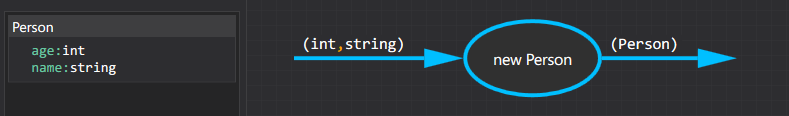
\includegraphics[width=.9\linewidth]{./img/roslyn_simpleOutput.png} 
	
	Die Generierung erzeugt folgenden Code:
	\begin{verbatim}
	public class Person
	{
	public string Name;
	public int Age;
	}
	
	public static Person NewPerson(int aint, string astring)
	{
	throw  new NotImplementedException();
	}
	\end{verbatim}
	
	Hat ein Output mehr als ein Datentyp und ist kein Stream und ist auch nicht optional, so
	wird das Ergebnis als Tupel über den Rückgabewert geliefert.
	
	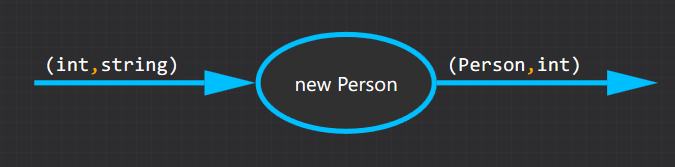
\includegraphics[width=.9\linewidth]{./img/roslyn_twoDatatypesOneOutput.png} 
	
	
	\begin{verbatim}
	TODO
	\end{verbatim}
	
	\item Outputs über Actions
	\label{sec:orgheadline36}
	Ob ein Ausgang über ein Action realisert wird, wird indirekt dadurch
	festgelegt, dass ein Actionname angegeben wurde (Diese Regel wurde im
	Rahmen dieser Anwendung so festgelegt). Ausgänge müssen nicht zwingend mit
	der Anzahl an Aufrufe der Funktionseinheit übereinstimmen. Ein Action muss
	nicht aufgrufen werden, oder kann bei einem einzigen Aufruf der Funktionseinheit auch
	mehrmals aufgerufen werden (der Beginn eines Streams). 
	
	Sobald auch eine Funktionseinheit mehrere Ausgänge hat, diese jedoch nicht
	Optional sind, werden diese jedoch trotzdem als Actions realisiert, selbst wenn sie kein
	Actionname zugeordnet bekommen haben. Der Name des Actions wird dann
	automatisch generiert. (Fussnote: Durch Analyse der Datentypen. Ein
	(Person) wird dann zu einem onPerson. Ein () wird zu einem continueWith. 
	
	Durch diese Entscheidungen gibt es keine invaliden Kombinationen an
	Ausgängen einer Funktionseinheit.
	
	
	Werden alle Ausgänge mit Actions realisiert, entfällt der Rückgabewert in diesem Fall.
	Die Input-Daten werden in der Signature zuerst aufgelistet, anschließend die Actions.
	
	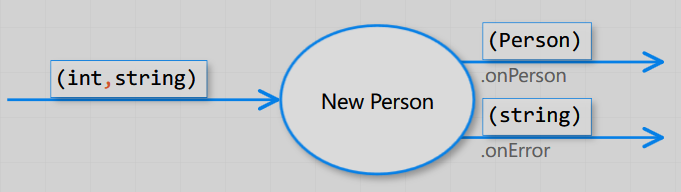
\includegraphics[width=.9\linewidth]{./img/roslyn_multipleOutputs.png} 
	
	\begin{verbatim}
	public static void NewPerson(int aint, string astring, Action<Person> onPerson, Action<string> onError)
	{
	throw  new NotImplementedException();
	}
	\end{verbatim}
	\item Streams
	\label{sec:orgheadline37}
	Stream werden ananlog zu den optionalen Outputs generiert, mit einer Ausnahme: 
	Sind ist sowohl der Input als auch der Output ein Stream und ist der Actionname
	des Outputs nicht angegeben, so wird davon ausgegangen, dass für jeden
	Datentyp der in die Funktionseinheit hineinfließt auch einer 
	herausfließt. Somit kann auf eine Action verzichtet werden und der
	Rückgabewert als Output genutzt werden. Was eine einfachers Verwenden
	dieser Funktionseinheit im Code zur Auswirkung hat.
	
	
	\includegraphics[width=.9\linewidth]{./img/roslyn_Stream.png} 
	
	
	\begin{verbatim}
	TODO
	\end{verbatim}
	
	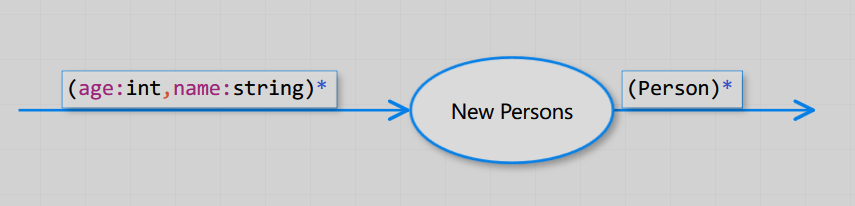
\includegraphics[width=.9\linewidth]{./img/roslyn_StreamStream.png} 
	
	\begin{verbatim}
	TODO
	\end{verbatim}
	
	
	(Fussnote)
	Das vorhandensein von einem Inputstream und einem Outputstream bedeutet nicht zwingend , dass für jeden Input auch ein
	Output erzeugt wird. Die Notation unterscheidet beide Fälle nicht. 
	Deswegen die Lösung über eine Vergabe eines Actionames als Kompromiss.
	Wenn der Benutzer ein Actioname angibt, wird indirekt davon ausgegangen,
	das die Inputs- und Outputstreams nicht übereinstimmen, anderseits wird
	davon ausgegangen (Dieses Verhalten muss dem Benutzer bewusst sein).
	
	Ob dieses Entscheidung richtig ist müsste  noch in der Praxis erprobt werden. Stellt sich heraus,
	dass das schlecht ist, so müsste man über eine Anpassung der Notation
	nachdenken.
	
	
	
	\item TDD
	\label{sec:orgheadline38}
	
	\item Codeauschnitte
	\label{sec:orgheadline39}
	
	\item DatanameParser
	\label{sec:orgheadline40}
\end{enumerate}
\subsubsection{Kleiner Einblick in die API von Roslyn}
\label{sec:orgheadline43}
Das Projekt Rosyln von Microsoft ist ein .NET-Compiler, der eine API bietet, um beliebigen C\#-Quelltext zu erstellten,
zu analysieren und zu modifizieren.

Das hier verwendetet Packet ist: Microsoft.CodeAnalysis

Der Datentypen auf dem die Methoden zum Erstellen von Code arbeitet lautet:
\texttt{SyntaxNode} 

Diese SyntaxNodes werden von einem SyntaxGenerator erstellt werden.
Diese muss beim Initialsieren konfiguriert werden.

\begin{verbatim}
var workspace = new AdhocWorkspace();
// Get the SyntaxGenerator for the specified language
var generator = SyntaxGenerator.GetGenerator(workspace, LanguageNames.CSharp);
\end{verbatim}


Das Erstellen eines Ausdruckes, Klasse oder Methode mit Hilfe von Methoden
des SyntaxGenerators lieferen am Ende immer eine SyntaxNode zurück.
Beim Erstellen einer Methode oder Klasse kann der Inhalt des Scopes durch
ein Array von SyntaxNodes bestimmt werden.

Nachfolgend ein einfaches Beispiel zum erstellen von einem
benutzerdefinierten Datentyp.

\begin{enumerate}
	\item Erzeugung eines Datentypen als einfaches Beispiel
	\label{sec:orgheadline42}
	
	\begin{verbatim}
	var fieldAlter = generator.FieldDeclaration(
	name: "Alter",
	type: generator.TypeExpression(SpecialType.System_Int32),
	accessibility: Accessibility.Public);
	
	var fieldName = generator.FieldDeclaration(
	name: "Name",
	type: generator.TypeExpression(SpecialType.System_String),
	accessibility: Accessibility.Public);
	
	
	var allFields =  new[] {fieldName, fieldAlter};
	
	
	// Generate the class
	var classDefinition = Generator.ClassDeclaration(
	"Person", 
	typeParameters: null,
	accessibility: Accessibility.Public,
	modifiers: DeclarationModifiers.None,
	baseType: null,
	interfaceTypes: null,
	members:allFields
	);
	\end{verbatim}
	
	Um am Ende den Code in Form eines Strings zu erhalten muss auf die oberstere
	SyntaxNode folgende beide Methoden aufgerufen werden:
	
	\begin{verbatim}
	var code = classDefinition.NormalizeWhitespace().ToFullString();
	\end{verbatim}
\end{enumerate}

\subsubsection{Erzeugung der Integration-Bodies}
\label{sec:orgheadline51}

\begin{enumerate}
	\item Terminologie
	\label{sec:orgheadline44}
	Integration und Sub-Funktionseinheit. Eine Integration kann nicht nur aus
	Operationen bestehen, sonder auch aus anderen Integrationen bestehen.
	Leider gibt es hierfür keine Überbegriff für beide.
	Da im in diese Kapitel jedoch öfters von Funktionseinheiten innerhalb einer
	Integration die Rede sein wird, muss hierfür ein Überbegriff eingeführt
	werden. Funktionseinheiten, die sich in einer Integration befinden, werden
	nachfolgend als Sub-Funktonseinheiten bezeichnet.
	
	\item Die Herangehensweise
	\label{sec:orgheadline45}
	
	Die automatische Erzeugung eines Integration ist die komplexeste Aufgabe in
	diesem Projekt. Um die Aufgabe überschaubar zu halten, wurde diese im groben in
	zwei Teileaufgaben zerteilt: die Analyse und die Generierung.
	Die Analyse besteht wiederum aus unterschiedlichen Methoden, die jeweils das
	Flow Design auf eine bestimme Sache analysieren und das Ergebnis in ein Objekt
	abspeichern. Diese Objekt wurde als \texttt{IntegrationBody} bezeichnet.
	Diese beinhaltet alle Informationen aus der Analyse. Am Ende wird dieses Objekt
	der Generierungsmethode Übergeben, die anhand diesem den Code erzeugt.
	
	\begin{verbatim}
	public static SyntaxNode[] GenerateIntegrationBody(SyntaxGenerator generator, MainModel mainModel,
	FunctionUnit integration )
	{
	// integrationbody object for storing analysed and generated information
	var integrationBody = IntegrationAnalyser.CreateNewIntegrationBody(mainModel.Connections, integration);
	AddIntegrationInputParameterToLocalScope(integrationBody, integration);
	
	// analyse data flow before generation 
	IntegrationAnalyser.AnalyseParameterDependencies(integrationBody);
	IntegrationAnalyser.AnalyseLambdaBodies(integrationBody, mainModel);
	IntegrationAnalyser.AnalyseMatchingOutputOfIntegration(integrationBody, mainModel);
	IntegrationAnalyser.AnalyseReturnToLocalReturnVariable(integrationBody, mainModel);
	
	// generation
	var result = new List<SyntaxNode>();
	integrationBody.Generator = generator;
	GenerateBody(integrationBody, result.Add);
	
	return result.ToArray();
	}
	\end{verbatim}
	
	\item Analyse des Flow Design
	\label{sec:orgheadline49}
	\begin{enumerate}
		\item AnalyseParameterDependencies
		\label{sec:orgheadline46}
		Da die Pipe-Notation unterstützt wird, reicht es nicht einfache aus die Daten
		aus den Datenflüssen zu nehmen, die direkt in die akutelle
		Funktionseinheit fließen. Stattdessen muss der Fluss rückwärts
		traversiert werden und auf Übereinstimmungen untersucht werden.
		Für jede Sub-Funktionseinheit muss diese Analyse durchgeführt werden.
		Für jeden Input-Datentyp jeder Funktioneinheit wird das Ergebnis gespeichert. Das Ergebnis beinhaltet ob der Datentyp überhaupt gefunden
		wurde, ob er im Input der Integration gefunden wurde, oder ob er aus einer
		anderen Sub-Funktionseinheit innerhalb des Datenflusses stammt. 
		Außerdem wird die gefundene DataStreamDefinition gespeichert, in der die
		Daten gefunden wurden. Ein Aufruf einer Sub-Funktionseinheit kann nur generiert werden, wenn alle Datentypen gefunden
		wurden.
		
		\item AnalyseLambdaBodies
		\label{sec:orgheadline47}
		Manche optionale Datenflüsse oder Stream werden über Actions realisiert.
		Das bedeutet, dass sich alle nachflogenden Funktionseinheiten innerhalb
		des Lambda-Ausdruckes befinden müssen. Die Analyse speichert das Ergebnis
		in folgender Form ab. 
		
		\begin{verbatim}
		public class LambdaBody
		{
		public DataStreamDefinition InsideLambdaOf;
		public FunctionUnit FunctionUnit;
		}
		\end{verbatim}
		
		Da die LambdaBody-Objekte in der Reihenfolge im IntegrationBody abgelegt
		werden, in der sie im Flow Design vorkommen, kann daraus auch später die
		Reihenfolge der zu generierenden Methoden abgeleitet werden.
		
		
		Für jede Funktionseinheit wird solch ein Objekt angelegt, auch wenn es
		nicht innerhalb eines Lambdas vorkommt. Ist das der Fall, so ist der Wert
		\texttt{InsideLambdaOf} \texttt{null} . Alle Funktionseinheiten für die dieser Wert
		\texttt{null} ist, befinden sich somit direkt im Scope der Integration und nicht
		innerhalb eines Lambdas.
		
		\item AnalyseMatchingOutputOfIntegration
		\label{sec:orgheadline48}
		Hat die Integration einen Output der als Action realisert werden muss, so
		muss herausgefunden werden, welche Funtionseinheiten im Datenfluss diesen
		Output erzeugt bedienen. Dabei werden die Implementierungs-Stile der
		beiden übereinstimmenden Ausgänge mit abgepeichert. Später bei der
		Generierung gibt es somit drei Möglichkeiten:
		\begin{itemize}
			\item Beide sind Actions:
			Die Action der Integration wird direkt an die Sub-Funktionseinheit
			weitergereicht. Dadurch erlaubt man einer Sub-Funktionseinheit das
			Aufrufen des Ausgang der Integration.
			\item Integrationsausgang ist Action, Sub-Funktionseinheitsausgang ist
			Returnwert 
			Die Action wird aufgerufen und die Methode wird direkt in diese
			hingeschrieben
			\item Integrationsausgang ist Returnwert, Sub-Funktionseinheitsausgang ist
			Action.
			Eine lokale Variable muss vorher angelegt werden und mit \texttt{null}
			initalisiert werden. Danach wird innerhalb des Lambas des Actions diese
			Variable beschrieben. Am Ende wird die lokale Varibale als Rückgabewert
			ausgegeben.
		\end{itemize}
	\end{enumerate}
	
	
	
	\item Datenströme
	\label{sec:orgheadline50}
\end{enumerate}

\subsection{Generierung eines Diagrammes aus Code}
\label{sec:orgheadline53}
Aus zeitlichen Gründen, konnte die Generierung von einem Flow Design aus Code
nicht angegangen werden. 
Da sich das Model jedoch sauber getrennt von der GUI in
einem speraten Unterprojekt befindet, wäre es sicherlich möglich einen anderen
Studenten dies als Bachelorarbeit zu übergeben. So hätte dieser bereits eine
Möglichkeit seine Diagramme darzustellen, ohne sich sonderlich in die
Codebasis von dem gesamten Dexel-Projektes einarbeiten zu müssen.